% Options for packages loaded elsewhere
\PassOptionsToPackage{unicode}{hyperref}
\PassOptionsToPackage{hyphens}{url}
\PassOptionsToPackage{dvipsnames,svgnames,x11names}{xcolor}
%
\documentclass[
  a4paper,
  DIV=11,
  numbers=noendperiod]{scrreprt}

\usepackage{amsmath,amssymb}
\usepackage{setspace}
\usepackage{iftex}
\ifPDFTeX
  \usepackage[T1]{fontenc}
  \usepackage[utf8]{inputenc}
  \usepackage{textcomp} % provide euro and other symbols
\else % if luatex or xetex
  \usepackage{unicode-math}
  \defaultfontfeatures{Scale=MatchLowercase}
  \defaultfontfeatures[\rmfamily]{Ligatures=TeX,Scale=1}
\fi
\usepackage{lmodern}
\ifPDFTeX\else  
    % xetex/luatex font selection
\fi
% Use upquote if available, for straight quotes in verbatim environments
\IfFileExists{upquote.sty}{\usepackage{upquote}}{}
\IfFileExists{microtype.sty}{% use microtype if available
  \usepackage[]{microtype}
  \UseMicrotypeSet[protrusion]{basicmath} % disable protrusion for tt fonts
}{}
\usepackage{xcolor}
\setlength{\emergencystretch}{3em} % prevent overfull lines
\setcounter{secnumdepth}{5}
% Make \paragraph and \subparagraph free-standing
\makeatletter
\ifx\paragraph\undefined\else
  \let\oldparagraph\paragraph
  \renewcommand{\paragraph}{
    \@ifstar
      \xxxParagraphStar
      \xxxParagraphNoStar
  }
  \newcommand{\xxxParagraphStar}[1]{\oldparagraph*{#1}\mbox{}}
  \newcommand{\xxxParagraphNoStar}[1]{\oldparagraph{#1}\mbox{}}
\fi
\ifx\subparagraph\undefined\else
  \let\oldsubparagraph\subparagraph
  \renewcommand{\subparagraph}{
    \@ifstar
      \xxxSubParagraphStar
      \xxxSubParagraphNoStar
  }
  \newcommand{\xxxSubParagraphStar}[1]{\oldsubparagraph*{#1}\mbox{}}
  \newcommand{\xxxSubParagraphNoStar}[1]{\oldsubparagraph{#1}\mbox{}}
\fi
\makeatother

\usepackage{color}
\usepackage{fancyvrb}
\newcommand{\VerbBar}{|}
\newcommand{\VERB}{\Verb[commandchars=\\\{\}]}
\DefineVerbatimEnvironment{Highlighting}{Verbatim}{commandchars=\\\{\}}
% Add ',fontsize=\small' for more characters per line
\usepackage{framed}
\definecolor{shadecolor}{RGB}{241,243,245}
\newenvironment{Shaded}{\begin{snugshade}}{\end{snugshade}}
\newcommand{\AlertTok}[1]{\textcolor[rgb]{0.68,0.00,0.00}{#1}}
\newcommand{\AnnotationTok}[1]{\textcolor[rgb]{0.37,0.37,0.37}{#1}}
\newcommand{\AttributeTok}[1]{\textcolor[rgb]{0.40,0.45,0.13}{#1}}
\newcommand{\BaseNTok}[1]{\textcolor[rgb]{0.68,0.00,0.00}{#1}}
\newcommand{\BuiltInTok}[1]{\textcolor[rgb]{0.00,0.23,0.31}{#1}}
\newcommand{\CharTok}[1]{\textcolor[rgb]{0.13,0.47,0.30}{#1}}
\newcommand{\CommentTok}[1]{\textcolor[rgb]{0.37,0.37,0.37}{#1}}
\newcommand{\CommentVarTok}[1]{\textcolor[rgb]{0.37,0.37,0.37}{\textit{#1}}}
\newcommand{\ConstantTok}[1]{\textcolor[rgb]{0.56,0.35,0.01}{#1}}
\newcommand{\ControlFlowTok}[1]{\textcolor[rgb]{0.00,0.23,0.31}{\textbf{#1}}}
\newcommand{\DataTypeTok}[1]{\textcolor[rgb]{0.68,0.00,0.00}{#1}}
\newcommand{\DecValTok}[1]{\textcolor[rgb]{0.68,0.00,0.00}{#1}}
\newcommand{\DocumentationTok}[1]{\textcolor[rgb]{0.37,0.37,0.37}{\textit{#1}}}
\newcommand{\ErrorTok}[1]{\textcolor[rgb]{0.68,0.00,0.00}{#1}}
\newcommand{\ExtensionTok}[1]{\textcolor[rgb]{0.00,0.23,0.31}{#1}}
\newcommand{\FloatTok}[1]{\textcolor[rgb]{0.68,0.00,0.00}{#1}}
\newcommand{\FunctionTok}[1]{\textcolor[rgb]{0.28,0.35,0.67}{#1}}
\newcommand{\ImportTok}[1]{\textcolor[rgb]{0.00,0.46,0.62}{#1}}
\newcommand{\InformationTok}[1]{\textcolor[rgb]{0.37,0.37,0.37}{#1}}
\newcommand{\KeywordTok}[1]{\textcolor[rgb]{0.00,0.23,0.31}{\textbf{#1}}}
\newcommand{\NormalTok}[1]{\textcolor[rgb]{0.00,0.23,0.31}{#1}}
\newcommand{\OperatorTok}[1]{\textcolor[rgb]{0.37,0.37,0.37}{#1}}
\newcommand{\OtherTok}[1]{\textcolor[rgb]{0.00,0.23,0.31}{#1}}
\newcommand{\PreprocessorTok}[1]{\textcolor[rgb]{0.68,0.00,0.00}{#1}}
\newcommand{\RegionMarkerTok}[1]{\textcolor[rgb]{0.00,0.23,0.31}{#1}}
\newcommand{\SpecialCharTok}[1]{\textcolor[rgb]{0.37,0.37,0.37}{#1}}
\newcommand{\SpecialStringTok}[1]{\textcolor[rgb]{0.13,0.47,0.30}{#1}}
\newcommand{\StringTok}[1]{\textcolor[rgb]{0.13,0.47,0.30}{#1}}
\newcommand{\VariableTok}[1]{\textcolor[rgb]{0.07,0.07,0.07}{#1}}
\newcommand{\VerbatimStringTok}[1]{\textcolor[rgb]{0.13,0.47,0.30}{#1}}
\newcommand{\WarningTok}[1]{\textcolor[rgb]{0.37,0.37,0.37}{\textit{#1}}}

\providecommand{\tightlist}{%
  \setlength{\itemsep}{0pt}\setlength{\parskip}{0pt}}\usepackage{longtable,booktabs,array}
\usepackage{calc} % for calculating minipage widths
% Correct order of tables after \paragraph or \subparagraph
\usepackage{etoolbox}
\makeatletter
\patchcmd\longtable{\par}{\if@noskipsec\mbox{}\fi\par}{}{}
\makeatother
% Allow footnotes in longtable head/foot
\IfFileExists{footnotehyper.sty}{\usepackage{footnotehyper}}{\usepackage{footnote}}
\makesavenoteenv{longtable}
\usepackage{graphicx}
\makeatletter
\def\maxwidth{\ifdim\Gin@nat@width>\linewidth\linewidth\else\Gin@nat@width\fi}
\def\maxheight{\ifdim\Gin@nat@height>\textheight\textheight\else\Gin@nat@height\fi}
\makeatother
% Scale images if necessary, so that they will not overflow the page
% margins by default, and it is still possible to overwrite the defaults
% using explicit options in \includegraphics[width, height, ...]{}
\setkeys{Gin}{width=\maxwidth,height=\maxheight,keepaspectratio}
% Set default figure placement to htbp
\makeatletter
\def\fps@figure{htbp}
\makeatother
% definitions for citeproc citations
\NewDocumentCommand\citeproctext{}{}
\NewDocumentCommand\citeproc{mm}{%
  \begingroup\def\citeproctext{#2}\cite{#1}\endgroup}
\makeatletter
 % allow citations to break across lines
 \let\@cite@ofmt\@firstofone
 % avoid brackets around text for \cite:
 \def\@biblabel#1{}
 \def\@cite#1#2{{#1\if@tempswa , #2\fi}}
\makeatother
\newlength{\cslhangindent}
\setlength{\cslhangindent}{1.5em}
\newlength{\csllabelwidth}
\setlength{\csllabelwidth}{3em}
\newenvironment{CSLReferences}[2] % #1 hanging-indent, #2 entry-spacing
 {\begin{list}{}{%
  \setlength{\itemindent}{0pt}
  \setlength{\leftmargin}{0pt}
  \setlength{\parsep}{0pt}
  % turn on hanging indent if param 1 is 1
  \ifodd #1
   \setlength{\leftmargin}{\cslhangindent}
   \setlength{\itemindent}{-1\cslhangindent}
  \fi
  % set entry spacing
  \setlength{\itemsep}{#2\baselineskip}}}
 {\end{list}}
\usepackage{calc}
\newcommand{\CSLBlock}[1]{\hfill\break\parbox[t]{\linewidth}{\strut\ignorespaces#1\strut}}
\newcommand{\CSLLeftMargin}[1]{\parbox[t]{\csllabelwidth}{\strut#1\strut}}
\newcommand{\CSLRightInline}[1]{\parbox[t]{\linewidth - \csllabelwidth}{\strut#1\strut}}
\newcommand{\CSLIndent}[1]{\hspace{\cslhangindent}#1}

\KOMAoption{captions}{tableheading}
\makeatletter
\@ifpackageloaded{bookmark}{}{\usepackage{bookmark}}
\makeatother
\makeatletter
\@ifpackageloaded{caption}{}{\usepackage{caption}}
\AtBeginDocument{%
\ifdefined\contentsname
  \renewcommand*\contentsname{Table of contents}
\else
  \newcommand\contentsname{Table of contents}
\fi
\ifdefined\listfigurename
  \renewcommand*\listfigurename{List of Figures}
\else
  \newcommand\listfigurename{List of Figures}
\fi
\ifdefined\listtablename
  \renewcommand*\listtablename{List of Tables}
\else
  \newcommand\listtablename{List of Tables}
\fi
\ifdefined\figurename
  \renewcommand*\figurename{Figure}
\else
  \newcommand\figurename{Figure}
\fi
\ifdefined\tablename
  \renewcommand*\tablename{Table}
\else
  \newcommand\tablename{Table}
\fi
}
\@ifpackageloaded{float}{}{\usepackage{float}}
\floatstyle{ruled}
\@ifundefined{c@chapter}{\newfloat{codelisting}{h}{lop}}{\newfloat{codelisting}{h}{lop}[chapter]}
\floatname{codelisting}{Listing}
\newcommand*\listoflistings{\listof{codelisting}{List of Listings}}
\makeatother
\makeatletter
\makeatother
\makeatletter
\@ifpackageloaded{caption}{}{\usepackage{caption}}
\@ifpackageloaded{subcaption}{}{\usepackage{subcaption}}
\makeatother

\ifLuaTeX
  \usepackage{selnolig}  % disable illegal ligatures
\fi
\usepackage{bookmark}

\IfFileExists{xurl.sty}{\usepackage{xurl}}{} % add URL line breaks if available
\urlstyle{same} % disable monospaced font for URLs
\hypersetup{
  pdftitle={thesis2024},
  pdfauthor={Joana Belmiro},
  colorlinks=true,
  linkcolor={blue},
  filecolor={Maroon},
  citecolor={Blue},
  urlcolor={Blue},
  pdfcreator={LaTeX via pandoc}}


\title{thesis2024}
\author{Joana Belmiro}
\date{2024-12-25}

\begin{document}
\maketitle

\renewcommand*\contentsname{Table of contents}
{
\hypersetup{linkcolor=}
\setcounter{tocdepth}{2}
\tableofcontents
}

\setstretch{2}
\bookmarksetup{startatroot}

\chapter*{Preface}\label{preface}
\addcontentsline{toc}{chapter}{Preface}

\markboth{Preface}{Preface}

This is a Quarto book.

To learn more about Quarto books visit
\url{https://quarto.org/docs/books}.

\begin{Shaded}
\begin{Highlighting}[]
\DecValTok{1} \SpecialCharTok{+} \DecValTok{1}
\end{Highlighting}
\end{Shaded}

\begin{verbatim}
[1] 2
\end{verbatim}

\bookmarksetup{startatroot}

\chapter{Introduction}\label{introduction}

This is a book created from markdown and executable code.

See Knuth (1984) for additional discussion of literate programming.

\begin{Shaded}
\begin{Highlighting}[]
\DecValTok{1} \SpecialCharTok{+} \DecValTok{1}
\end{Highlighting}
\end{Shaded}

\begin{verbatim}
[1] 2
\end{verbatim}

\bookmarksetup{startatroot}

\chapter{Summary}\label{summary}

In summary, this book has no content whatsoever.

\begin{Shaded}
\begin{Highlighting}[]
\DecValTok{1} \SpecialCharTok{+} \DecValTok{1}
\end{Highlighting}
\end{Shaded}

\begin{verbatim}
[1] 2
\end{verbatim}

\bookmarksetup{startatroot}

\chapter{geochemistry}\label{geochemistry}

\section{X-ray diffraction (XRD)}\label{x-ray-diffraction-xrd}

Some text. Some other text. A bit more of text.

\section{Scanning electron microscopy and energy dispersive X-ray
spectroscopy
(SEM-EDS)}\label{scanning-electron-microscopy-and-energy-dispersive-x-ray-spectroscopy-sem-eds}

\section{Portable X-ray fluorescence
(pXRF)}\label{portable-x-ray-fluorescence-pxrf}

\begin{figure}

\centering{

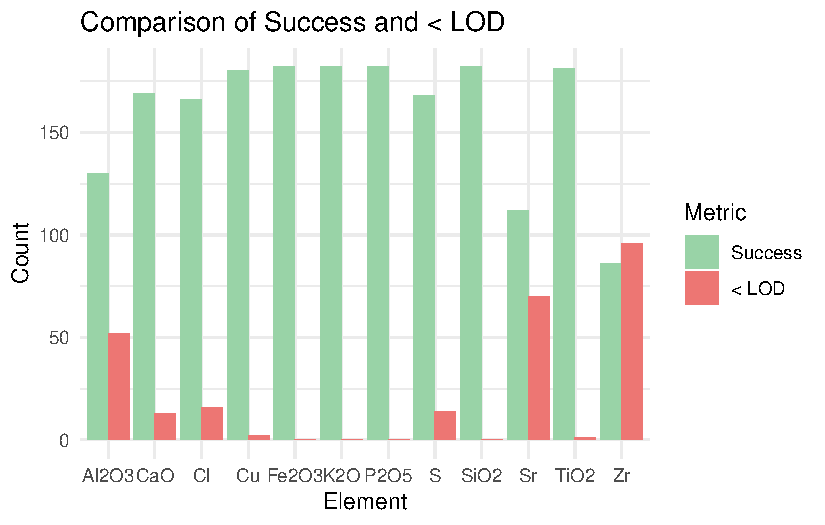
\includegraphics{geochemistry_files/figure-pdf/fig-lod-1.pdf}

}

\caption{\label{fig-lod-1}A barplot.}

\end{figure}%

\begin{figure}

\centering{

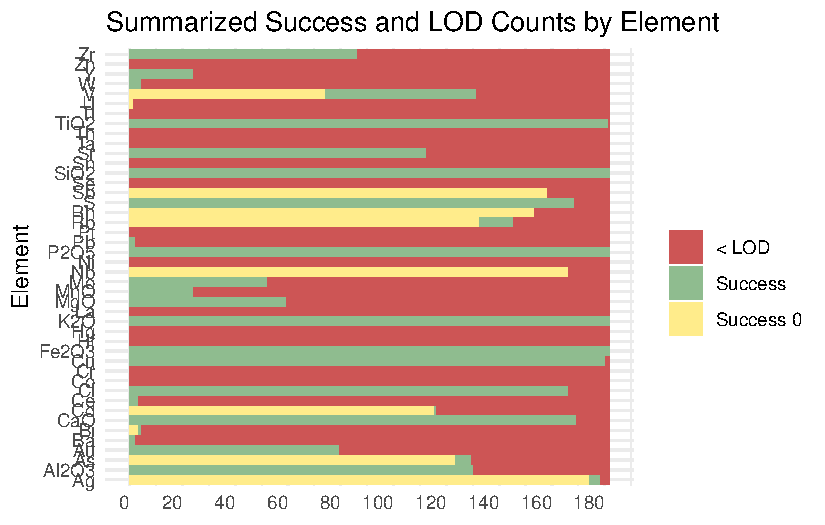
\includegraphics{geochemistry_files/figure-pdf/fig-lod-2.pdf}

}

\caption{\label{fig-lod-2}A barplot.}

\end{figure}%

\begin{verbatim}

Call:
PCA(X = df_scaled_alg, graph = FALSE) 


Eigenvalues
                       Dim.1   Dim.2   Dim.3   Dim.4   Dim.5   Dim.6   Dim.7
Variance               2.419   1.842   1.009   0.800   0.663   0.151   0.116
% of var.             34.558  26.319  14.408  11.424   9.477   2.154   1.660
Cumulative % of var.  34.558  60.877  75.284  86.708  96.186  98.340 100.000

Individuals (the 10 first)
          Dist    Dim.1    ctr   cos2    Dim.2    ctr   cos2    Dim.3    ctr
LJW   |  5.517 |  2.737  4.995  0.246 | -1.311  1.504  0.056 |  2.627 11.035
LJW.1 |  3.781 |  3.129  6.527  0.685 | -1.509  1.995  0.159 | -0.957  1.465
LJW.2 |  5.036 |  2.464  4.047  0.239 |  2.696  6.365  0.287 |  2.566 10.531
LJW.3 |  1.616 |  0.869  0.503  0.289 | -1.289  1.455  0.636 | -0.092  0.013
LJW.4 |  6.734 |  3.205  6.849  0.227 |  4.295 16.149  0.407 |  3.622 20.978
LJW.5 |  3.092 | -2.104  2.952  0.463 |  2.084  3.804  0.455 | -0.332  0.176
LJW.6 |  2.173 |  1.088  0.789  0.251 | -1.751  2.683  0.649 | -0.387  0.240
LJW.7 |  1.942 |  1.247  1.036  0.412 | -1.282  1.440  0.436 | -0.305  0.148
LJW.8 |  3.021 |  2.064  2.840  0.467 | -1.639  2.352  0.294 | -0.995  1.582
LJW.9 |  6.299 |  4.211 11.824  0.447 |  3.056  8.174  0.235 | -1.359  2.953
        cos2  
LJW    0.227 |
LJW.1  0.064 |
LJW.2  0.260 |
LJW.3  0.003 |
LJW.4  0.289 |
LJW.5  0.012 |
LJW.6  0.032 |
LJW.7  0.025 |
LJW.8  0.108 |
LJW.9  0.047 |

Variables
         Dim.1    ctr   cos2    Dim.2    ctr   cos2    Dim.3    ctr   cos2  
P2O5  |  0.805 26.793  0.648 |  0.490 13.038  0.240 | -0.148  2.184  0.022 |
S     |  0.659 17.966  0.435 |  0.491 13.067  0.241 | -0.154  2.358  0.024 |
Cl    |  0.360  5.358  0.130 |  0.474 12.190  0.225 |  0.611 37.034  0.374 |
K2O   |  0.667 18.400  0.445 | -0.675 24.757  0.456 | -0.141  1.971  0.020 |
CaO   |  0.081  0.270  0.007 |  0.596 19.287  0.355 | -0.379 14.249  0.144 |
TiO2  |  0.730 22.056  0.534 | -0.530 15.270  0.281 | -0.223  4.925  0.050 |
Fe2O3 |  0.471  9.157  0.222 | -0.210  2.391  0.044 |  0.613 37.279  0.376 |
\end{verbatim}

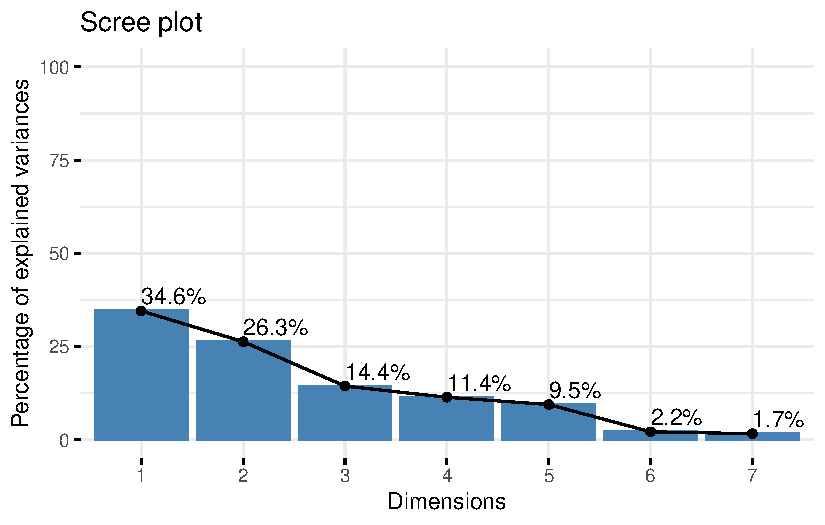
\includegraphics{geochemistry_files/figure-pdf/PCA-1.pdf}

\begin{verbatim}

Call:
PCA(X = df_scaled_nl, graph = FALSE) 


Eigenvalues
                       Dim.1   Dim.2   Dim.3   Dim.4   Dim.5   Dim.6
Variance               2.933   1.713   0.672   0.354   0.249   0.079
% of var.             48.885  28.546  11.197   5.901   4.157   1.314
Cumulative % of var.  48.885  77.431  88.628  94.529  98.686 100.000

Individuals (the 10 first)
          Dist    Dim.1    ctr   cos2    Dim.2    ctr   cos2    Dim.3    ctr
CPT   |  1.744 | -1.714  1.411  0.967 | -0.066  0.004  0.001 | -0.142  0.042
CPT.1 |  1.797 | -1.356  0.884  0.570 |  0.402  0.133  0.050 |  1.046  2.295
CPT.2 |  1.426 | -1.330  0.850  0.870 | -0.353  0.103  0.061 | -0.060  0.008
CPT.3 |  1.825 | -1.803  1.561  0.975 | -0.070  0.004  0.001 | -0.084  0.015
CPT.4 |  1.815 | -1.703  1.393  0.881 | -0.332  0.090  0.033 | -0.360  0.272
CPT.5 |  1.224 | -0.702  0.237  0.329 | -0.651  0.348  0.282 | -0.659  0.911
CPT.6 |  1.542 | -1.503  1.085  0.951 | -0.100  0.008  0.004 | -0.197  0.081
CPT.7 |  1.883 | -1.787  1.534  0.901 | -0.216  0.038  0.013 | -0.432  0.391
CPT.8 |  1.592 | -1.544  1.145  0.941 |  0.056  0.003  0.001 |  0.099  0.020
CPT.9 |  1.712 | -1.523  1.114  0.792 |  0.441  0.160  0.066 |  0.475  0.474
        cos2  
CPT    0.007 |
CPT.1  0.339 |
CPT.2  0.002 |
CPT.3  0.002 |
CPT.4  0.039 |
CPT.5  0.290 |
CPT.6  0.016 |
CPT.7  0.053 |
CPT.8  0.004 |
CPT.9  0.077 |

Variables
         Dim.1    ctr   cos2    Dim.2    ctr   cos2    Dim.3    ctr   cos2  
P2O5  |  0.668 15.194  0.446 |  0.591 20.375  0.349 | -0.119  2.094  0.014 |
K2O   |  0.836 23.802  0.698 | -0.463 12.504  0.214 | -0.073  0.791  0.005 |
TiO2  |  0.886 26.789  0.786 | -0.370  7.986  0.137 | -0.053  0.411  0.003 |
Fe2O3 |  0.844 24.304  0.713 | -0.237  3.278  0.056 |  0.110  1.797  0.012 |
Cu    |  0.411  5.761  0.169 |  0.632 23.299  0.399 |  0.637 60.406  0.406 |
S     |  0.349  4.150  0.122 |  0.747 32.557  0.558 | -0.481 34.501  0.232 |
\end{verbatim}

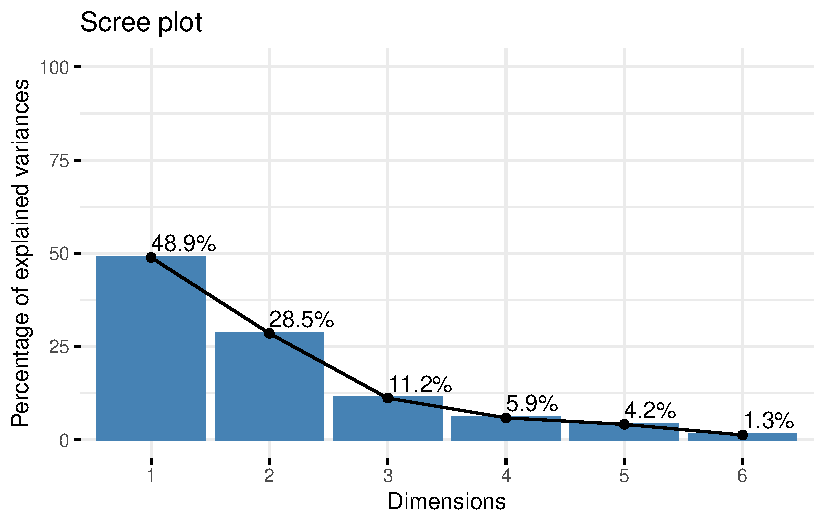
\includegraphics{geochemistry_files/figure-pdf/PCA-2.pdf}

\begin{verbatim}

Call:
PCA(X = df_scaled_comp, graph = FALSE) 


Eigenvalues
                       Dim.1   Dim.2   Dim.3   Dim.4   Dim.5   Dim.6
Variance               2.729   1.753   0.712   0.456   0.247   0.103
% of var.             45.477  29.222  11.871   7.600   4.121   1.709
Cumulative % of var.  45.477  74.699  86.570  94.170  98.291 100.000

Individuals (the 10 first)
          Dist    Dim.1    ctr   cos2    Dim.2    ctr   cos2    Dim.3    ctr
CPT   |  1.872 | -1.795  1.639  0.919 |  0.369  0.108  0.039 | -0.111  0.024
CPT.1 |  1.907 | -1.389  0.982  0.531 |  0.687  0.374  0.130 |  0.936  1.710
CPT.2 |  1.356 | -1.275  0.827  0.884 | -0.107  0.009  0.006 |  0.041  0.003
CPT.3 |  2.000 | -1.935  1.907  0.936 |  0.426  0.144  0.045 | -0.116  0.026
CPT.4 |  1.850 | -1.773  1.600  0.918 |  0.089  0.006  0.002 | -0.328  0.209
CPT.5 |  1.308 | -0.359  0.066  0.075 | -0.852  0.574  0.424 | -0.776  1.174
CPT.6 |  1.570 | -1.502  1.149  0.915 |  0.237  0.045  0.023 | -0.150  0.044
CPT.7 |  1.991 | -1.882  1.802  0.894 |  0.248  0.049  0.016 | -0.399  0.310
CPT.8 |  1.674 | -1.552  1.225  0.860 |  0.353  0.099  0.044 |  0.044  0.004
CPT.9 |  1.986 | -1.618  1.333  0.664 |  0.979  0.759  0.243 |  0.475  0.440
        cos2  
CPT    0.003 |
CPT.1  0.241 |
CPT.2  0.001 |
CPT.3  0.003 |
CPT.4  0.031 |
CPT.5  0.352 |
CPT.6  0.009 |
CPT.7  0.040 |
CPT.8  0.001 |
CPT.9  0.057 |

Variables
         Dim.1    ctr   cos2    Dim.2    ctr   cos2    Dim.3    ctr   cos2  
P2O5  |  0.663 16.108  0.440 |  0.620 21.955  0.385 | -0.190  5.080  0.036 |
K2O   |  0.712 18.598  0.507 | -0.630 22.626  0.397 | -0.108  1.653  0.012 |
TiO2  |  0.800 23.482  0.641 | -0.491 13.763  0.241 | -0.048  0.321  0.002 |
Fe2O3 |  0.751 20.672  0.564 | -0.247  3.491  0.061 |  0.295 12.221  0.087 |
Cu    |  0.463  7.866  0.215 |  0.576 18.943  0.332 |  0.617 53.383  0.380 |
S     |  0.602 13.273  0.362 |  0.581 19.222  0.337 | -0.441 27.342  0.195 |
\end{verbatim}

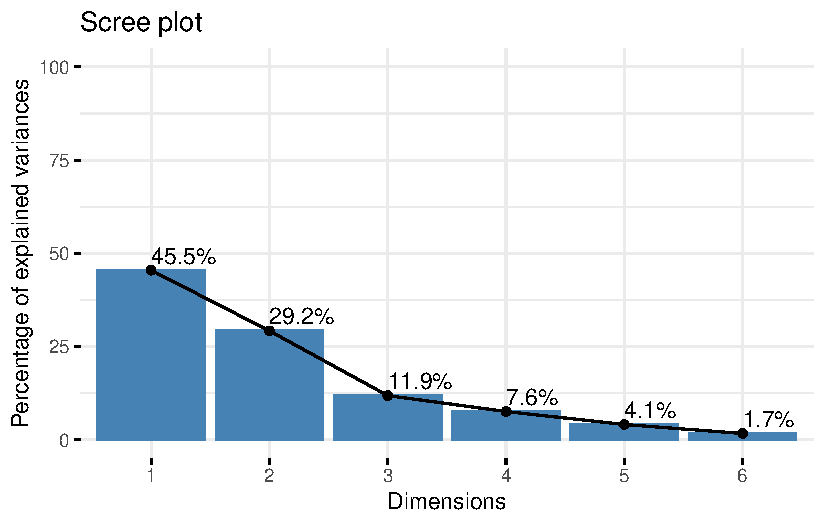
\includegraphics{geochemistry_files/figure-pdf/PCA-3.pdf}

\begin{verbatim}

Call:
PCA(X = df_scaled_comp2, graph = FALSE) 


Eigenvalues
                       Dim.1   Dim.2   Dim.3   Dim.4   Dim.5   Dim.6
Variance               3.074   1.638   0.687   0.329   0.237   0.035
% of var.             51.229  27.306  11.444   5.478   3.956   0.588
Cumulative % of var.  51.229  78.534  89.978  95.456  99.412 100.000

Individuals (the 10 first)
          Dist    Dim.1    ctr   cos2    Dim.2    ctr   cos2    Dim.3    ctr
LJW   |  3.502 |  1.688  0.997  0.232 | -0.419  0.115  0.014 |  0.306  0.147
LJW.1 |  1.452 |  1.128  0.445  0.604 |  0.594  0.232  0.168 | -0.644  0.649
LJW.2 |  2.521 |  0.866  0.262  0.118 |  1.892  2.350  0.563 | -1.389  3.020
LJW.3 |  0.560 |  0.044  0.001  0.006 | -0.390  0.100  0.485 | -0.313  0.153
LJW.4 |  3.148 |  1.069  0.400  0.115 |  2.767  5.026  0.773 | -0.431  0.290
LJW.5 |  1.545 | -1.026  0.368  0.441 |  0.339  0.076  0.048 | -1.094  1.876
LJW.6 |  0.899 |  0.196  0.013  0.048 | -0.082  0.004  0.008 | -0.832  1.084
LJW.7 |  1.453 | -0.219  0.017  0.023 | -0.853  0.478  0.345 |  0.961  1.445
LJW.8 |  0.819 |  0.167  0.010  0.041 | -0.546  0.196  0.445 |  0.524  0.430
LJW.9 |  6.112 |  1.021  0.365  0.028 |  4.521 13.412  0.547 |  3.411 18.220
        cos2  
LJW    0.008 |
LJW.1  0.197 |
LJW.2  0.303 |
LJW.3  0.313 |
LJW.4  0.019 |
LJW.5  0.502 |
LJW.6  0.857 |
LJW.7  0.437 |
LJW.8  0.410 |
LJW.9  0.311 |

Variables
         Dim.1    ctr   cos2    Dim.2    ctr   cos2    Dim.3    ctr   cos2  
P2O5  |  0.646 13.594  0.418 |  0.600 21.968  0.360 |  0.160  3.721  0.026 |
TiO2  |  0.921 27.594  0.848 | -0.316  6.092  0.100 |  0.052  0.399  0.003 |
K2O   |  0.889 25.723  0.791 | -0.371  8.410  0.138 |  0.114  1.903  0.013 |
Fe2O3 |  0.886 25.565  0.786 | -0.180  1.986  0.033 | -0.015  0.035  0.000 |
Cu    |  0.449  6.564  0.202 |  0.555 18.818  0.308 | -0.690 69.388  0.476 |
S     |  0.172  0.960  0.029 |  0.837 42.727  0.700 |  0.411 24.554  0.169 |
\end{verbatim}

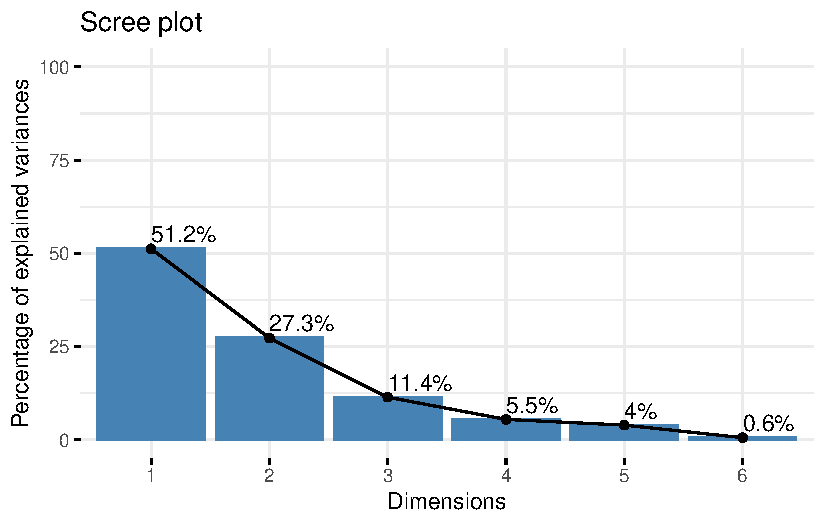
\includegraphics{geochemistry_files/figure-pdf/PCA-4.pdf}

\begin{figure}

\centering{

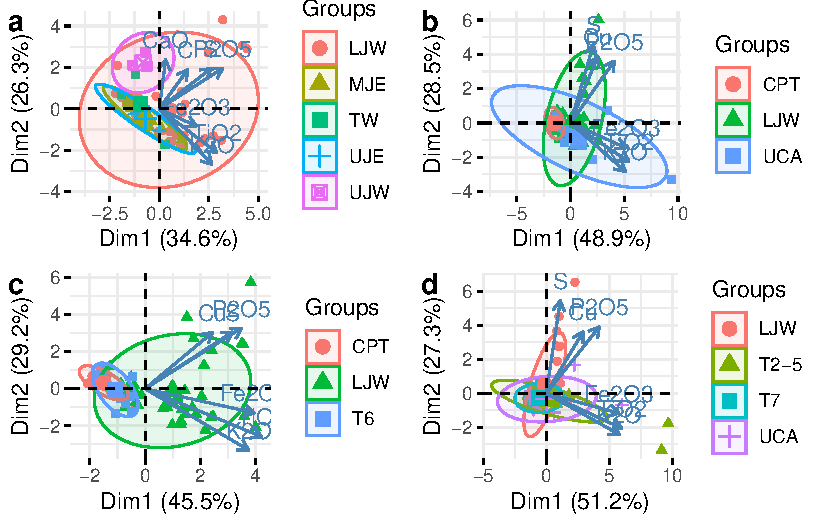
\includegraphics{geochemistry_files/figure-pdf/fig-pca-1.pdf}

}

\caption{\label{fig-pca}Several pcas}

\end{figure}%

\section{Methodology}\label{methodology}

For this experiment, a Bruker portable XRF Titan S1 was used in a
laboratory benchtop setup, using battery power (up to 25\% battery
charge then replaced by a fully charged battery). A validation run was
applied on two standard samples provided by Bruker and using the
standard calibration. Samples were scanned for 180 seconds each (90
seconds for the first phase for major elements and 90 seconds for the
second phase for minor elements), at least once, with several scans
applied to samples that showed macroscopic variability (e.g., areas with
different colours or translucency). The standard database from Bruker
was used, with the Geochem application and Dual Mining method. ** chert
samples were scanned, from several sources and chert types, both
geological and archaeological. After scanning, the scanned face was
measured (thickness and diameter), to guarantee a minimum thickness and
size was followed for each sample, since other studies have shown
thickness and size may impact the homogeneity of data collection and
results (Newlander et al. 2015). All samples, including their thickness
and diameter, can be found in table X. For geological samples, fresh,
flat surfaces were scanned, avoiding altered faces or cortex; whenever
necessary, the samples were prepared by breaking the nodules. The
samples were chosen to represent all varieties of chert identified in
the Algarve region, in the archaeological record of Vale Boi, but also
from other regions such as Central Portugal and South Spain, to allow
their comparison and test hypotheses made from macroscopic and
petrographic data. For archaeological samples, artefacts were chosen
from previously identified types (REF?), focusing on larger and flatter
morphologies, with the least degree of surface alterations possible.

The analysis and result reporting protocol was established following
previous studies, focusing on the accuracy of obtained data but also the
transparency and reproducibility of the results (Newlander et al. 2015;
Johnson et al. 2024). For further reproducibility and replicability, and
working towards the goal of open science (Johnson et al. 2024; Marwick
2017), the obtained raw pXRF results can be found online on our online
compendium (LINK).

\section{Results}\label{results}

The pXRF measured several major and minor elements, of which a small
amount returned values of 0 or were below the limit of detection
(\textless LOD). These were uranium (U), thorium (Th), bismuth (Bi),
thallium (Tl), mercury (Hg), platinum (Pt), tantalum (Ta), hafnium (Hf),
lanthanum (La), antimony (Sb), Tin (Sn), cadmium (Cd), rhodium (Rh),
niobium (Nb), selenium (Se), zinc (Zn), nickel (Ni), cobalt (Co) and
chromium (Cr). They were removed from the analysis based on their
nonexistence, although they can still be found in the raw pXRF results.

\bookmarksetup{startatroot}

\chapter*{References}\label{references}
\addcontentsline{toc}{chapter}{References}

\markboth{References}{References}

\phantomsection\label{refs}
\begin{CSLReferences}{1}{0}
\bibitem[\citeproctext]{ref-johnsonBestPracticesPublishing2024}
Johnson, Kimberly, Colin P. Quinn, Nathan Goodale, and Richard Conrey.
2024. {``Best Practices for Publishing pXRF Analyses.''} \emph{Advances
in Archaeological Practice} 12 (2): 156--62.
\url{https://doi.org/10.1017/aap.2024.6}.

\bibitem[\citeproctext]{ref-knuth84}
Knuth, Donald E. 1984. {``Literate Programming.''} \emph{Comput. J.} 27
(2): 97--111. \url{https://doi.org/10.1093/comjnl/27.2.97}.

\bibitem[\citeproctext]{ref-marwickComputationalReproducibilityArchaeological2017}
Marwick, Ben. 2017. {``Computational Reproducibility in Archaeological
Research: Basic Principles and a Case Study of Their Implementation.''}
\emph{Journal of Archaeological Method and Theory} 24 (2): 424--50.
\url{https://doi.org/10.1007/s10816-015-9272-9}.

\bibitem[\citeproctext]{ref-newlanderEmpiricalStudyEffect2015}
Newlander, Khori, Nathan Goodale, George T. Jones, and David G. Bailey.
2015. {``Empirical Study of the Effect of Count Time on the Precision
and Accuracy of pXRF Data.''} \emph{Journal of Archaeological Science:
Reports} 3 (September): 534--48.
\url{https://doi.org/10.1016/j.jasrep.2015.07.007}.

\end{CSLReferences}

\phantomsection\label{refs}
\begin{CSLReferences}{1}{0}
\bibitem[\citeproctext]{ref-johnsonBestPracticesPublishing2024}
Johnson, Kimberly, Colin P. Quinn, Nathan Goodale, and Richard Conrey.
2024. {``Best Practices for Publishing pXRF Analyses.''} \emph{Advances
in Archaeological Practice} 12 (2): 156--62.
\url{https://doi.org/10.1017/aap.2024.6}.

\bibitem[\citeproctext]{ref-knuth84}
Knuth, Donald E. 1984. {``Literate Programming.''} \emph{Comput. J.} 27
(2): 97--111. \url{https://doi.org/10.1093/comjnl/27.2.97}.

\bibitem[\citeproctext]{ref-marwickComputationalReproducibilityArchaeological2017}
Marwick, Ben. 2017. {``Computational Reproducibility in Archaeological
Research: Basic Principles and a Case Study of Their Implementation.''}
\emph{Journal of Archaeological Method and Theory} 24 (2): 424--50.
\url{https://doi.org/10.1007/s10816-015-9272-9}.

\bibitem[\citeproctext]{ref-newlanderEmpiricalStudyEffect2015}
Newlander, Khori, Nathan Goodale, George T. Jones, and David G. Bailey.
2015. {``Empirical Study of the Effect of Count Time on the Precision
and Accuracy of pXRF Data.''} \emph{Journal of Archaeological Science:
Reports} 3 (September): 534--48.
\url{https://doi.org/10.1016/j.jasrep.2015.07.007}.

\end{CSLReferences}

\cleardoublepage
\phantomsection
\addcontentsline{toc}{part}{Appendices}
\appendix

\chapter{Supplementary materials 1}\label{supplementary-materials-1}

Some supplementary materials.




\end{document}
